\scanpage{65}
% archive foliation: 64
\diagram{\begin{tikzcd}
\pi_1(X\times Y)\arrow[r,"\uline{\text{surj}}"]&\pi_1(X)\times\pi_1(Y)
\end{tikzcd}}
\figure{
\begin{tikzpicture}\draw (0,0)--(.3,.4);\draw (0,.4)--(.3,0);\draw (1.1,.4)--(1.4,0);\end{tikzpicture}}

\diagram{\begin{tikzcd}
X\arrow[d]&Z\arrow[l,phantom,"\supset" description]\\Y&
\end{tikzcd}}
\diagram{\begin{tikzcd}
\pi_1(\unsure{Z})\arrow[r,no head]&\pi_1(X)\arrow[r,no head]&\pi_1(Y)
\end{tikzcd}}

\diagram{\begin{tikzcd}
X''\arrow[d,shift left=.4ex]\arrow[d,shift right=.4ex]\\
X'\arrow[d]\\X\arrow[d]\\ \cdot
\end{tikzcd}}
\figure{\begin{tikzpicture}
\draw[line width=2pt] (0,0)--(0,1.8);
\draw (-3.3,-1.0)--(-3.65,-.05);
\draw (-3.65,-1.0)--(-3.3,.05);
\fill (-3.48,-.48) circle (.065);
\draw (-2.7,-1.45)..controls (-3,-1.5) and (-2.9,.85)..(-2.72,.82)
..controls (-2.48,.80) and (-2.55,-1.5)..(-2.7,-1.45);
\end{tikzpicture}}

\diagram{\begin{tikzcd}
X\arrow[d]\arrow[r,phantom,"\subset" description]&\widehat X\arrow[d]&\text{normaux}\\
X_0\arrow[r,phantom,"\subset" description]&\widehat X_0&\unsure{\text{pts réguliers}}
\end{tikzcd}}
\figure{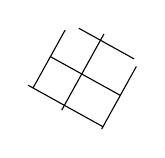
\begin{tikzpicture}[rotate=-29,scale=.7]
\draw (0,0)--(0,1.2); \draw (.65,-.1)--(.65,1.48);
\draw (1.45,-.05)--(1.45,1.25);
\draw (-.1,0)--(1.45,0); \draw (0,.65)--(1.45,.65);
\draw (.2,1.35)--(1.35,1.35);
\end{tikzpicture}}

\diagram{\begin{tikzcd}
Y'\arrow[r,no head]\arrow[d]&X'\arrow[d]\\
Y\arrow[r,phantom,"\subset" description]&X\arrow[d]\\
&P^r
\end{tikzcd}}
\diagram{\begin{tikzcd}
X'\arrow[r,phantom,"\subset" description]\arrow[d]&\unsure{\widehat X'|\overline X'}\arrow[d]\\
X\arrow[r,phantom,"\subset" description]\arrow[d]&\overline X\arrow[dl]\\
P^r&
\end{tikzcd}}
\diagram{\begin{tikzcd}
Y\arrow[r]\arrow[d]&X\arrow[d]\\
H\arrow[r]&P^r\\
/ K&/ k
\end{tikzcd}}
\diagram{\begin{tikzcd}\pi_1(Y)\arrow[r]&\pi_1(X)\end{tikzcd}}
$X$ normal

\diagram{\begin{tikzcd}
\pi_1(Y)\arrow[r,"\text{surj??}"]&\pi_1(X)
\end{tikzcd}}
\[
\pi_1(X)
\]
\figure{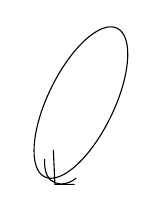
\begin{tikzpicture}
\draw[rotate around={-26:(0,0)}] (0,0) ellipse (.42 and 1.05);
\draw (-.46,-.72)..controls (-.48,-1.07) and (-.22,-1.09)..(-.06,-.96);
\draw (-.35,-.6)--(-.33,-1.04)--(-.08,-1.04);
\end{tikzpicture}}
\deleted{\diagram{\begin{tikzcd}
\pi_1(Y)\arrow[r]&\pi_1(X)&\pi_1(X-Y)\arrow[l]
\end{tikzcd}}}
